\section{Architectural Design}

\subsection{High level components and interactions}
The following block diagram describes the overall solution design by giving an high-level perspective of all main application roles. In particular, it makes easy to understand the partition of software service components across the solution realm and their interaction mechanisms through internal subsystems interfaces.

\begin{figure} [h!]
\centering
\includegraphics[scale=0.66]{{Figures/Architecture.png}}
\label{fig:Architecture}
\end{figure}

% \begin{wrapfigure}{r}{5.5cm}
% \caption{A wrapped figure going nicely inside the  text.}\label{wrap-fig:1}
% \includegraphics[width=5.5cm]{Figures/Architecture.png}
% \end{wrapfigure} 
%------------------------------------------
% {\lipsum[2-3]
% \par
% Figure~\ref{wrap-fig:1} is a wrapped figure.}


\begin{itemize}
\item{\textbf{Client side applications}}\newline
Represent the pool of user interactive applications made of both mobile applications running on user owned devices and onboard ride assistants running on the onboard infotainment devices of PowerEnJoy Cars.
\item{\textbf{Vehicle management platforms}}\newline
Represent the pool of embedded controllers devoted to remotely interfacing the vehicle hardware.

\item{\textbf{Front-end service roles}}
\begin{itemize}
\item{\textbf{Client Worker}}\newline
A single Client Worker node acts as a proxy between any remote interactive client and back-end components. In other words, it exposes all interfaces needed by any application the end user directly interacts with to allow decoupling from core service feature components, avoiding any client technology-dependent issue to be addressed by back-end design decisions. It is able to validate an existing authentication token avoiding redundant messaging to the back-end. It also provides access to static/cached resources and it's designed to be fully stateless, allowing automatic/on-demand scale-up of nodes instances to distribute workload across, dramatically increasing reliability and performance. A CW node can return execution results to remote clients both in synchronous (request/response) or asynchronous mode (event/notification).
\item{\textbf{Vehicle Worker}}\newline
A single Vehicle Worker node acts as a proxy between any remote supported vehicle platform and back-end components. In other words, it exposes all interfaces needed by any supported vehicle to allow decoupling from core service feature components, avoiding any platform-dependent issue to be addressed by back-end design decisions. it's designed to manage and keep track of an huge number of status/telemetry updates. Inside a VW node, updates from multiple different vehicles are stored until expiration and timestamped. When an event is triggered by a new vehicle the node registers itself to the back-end as the handler of that vehicle. This way we are still allowing automatic/on-demand scale-up of nodes instances to distribute workload across, dramatically increasing reliability and performance. A VW node works only in asynchronous mode (event/notification) w.r.t. the remote vehicle.
\item{\textbf{Elastic load balancing request router}}\newline
Available from any common cloud provider. Provides automatic scale-uo/-down of nodes instances based on their resources utilization and redirects request messages to nodes guaranteeing a fair workload distribution across them.
\item{\textbf{Elastic load balancing event hub}}\newline
Available from any common cloud provider. Provides automatic scale-uo/-down of nodes instances based on their resources utilization and manages to forward an huge number of event messages to nodes guaranteeing a fair workload distribution across them.
\item{\textbf{Elastic async push messages dispatcher}}\newline
Available from any common cloud provider. Provides efficient queuing of large number of messages to dispatch to multiple groups of targets. It also takes care of creating and keeping up network notification channels.
\end{itemize}

\item{\textbf{Back-end service roles}}
\begin{itemize}
\item{\textbf{Service Back-end Logic Worker}}\newline
TEXT
\item{\textbf{Elastic load balancing service bus}}\newline
TEXT
\item{\textbf{User Account Data}}\newline
TEXT
\item{\textbf{Configuration Data}}\newline
TEXT
\item{\textbf{Single Zone Data}}\newline
TEXT
\end{itemize}
\end{itemize}

\subsection{Component view}

\subsubsection{Service Back-end Logic}
\begin{figure} [h!]
\centering
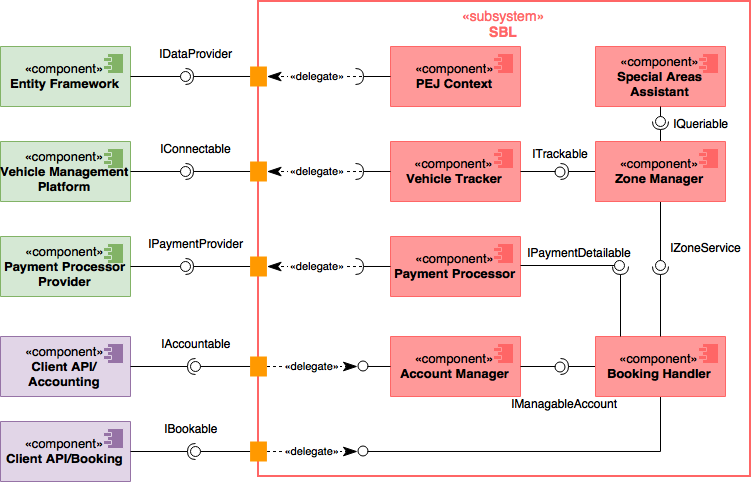
\includegraphics[scale=0.5]{{Figures/Component_Diagram/SBL.png}}
\label{fig:SBL}
\end{figure}
EXPLANATION TEXT
%Add \newpage here if necessary
\newpage

\subsubsection{Mobile App}
\begin{figure} [h!]
\centering
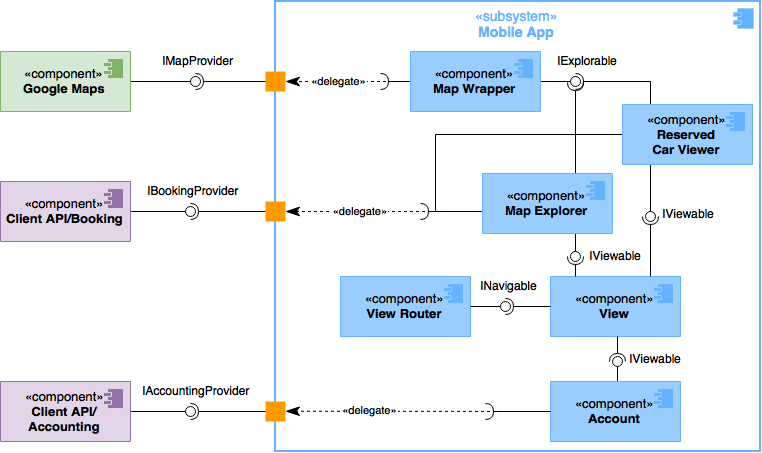
\includegraphics[scale=0.5]{{Figures/Component_Diagram/MobileApp.png}}
\label{fig:MobileApp}
\end{figure}
EXPLANATION TEXT
%Add \newpage here if necessary
\newpage

\subsubsection{Car App}
\begin{figure} [h!]
\centering
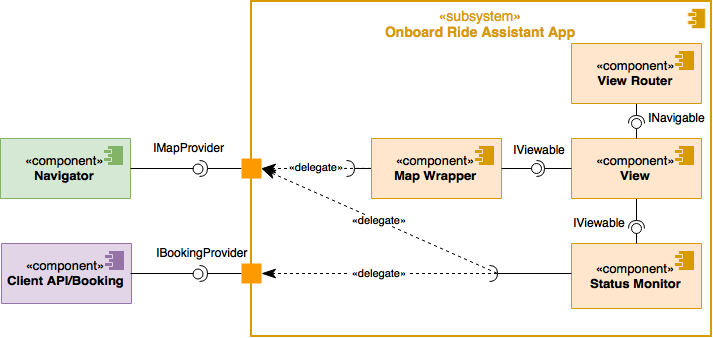
\includegraphics[scale=0.5]{{Figures/Component_Diagram/CarApp.png}}
\label{fig:CarApp}
\end{figure}
EXPLANATION TEXT
%Add \newpage here if necessary
\newpage

\subsection{Deployment view}
\begin{figure} [h!]
\centering
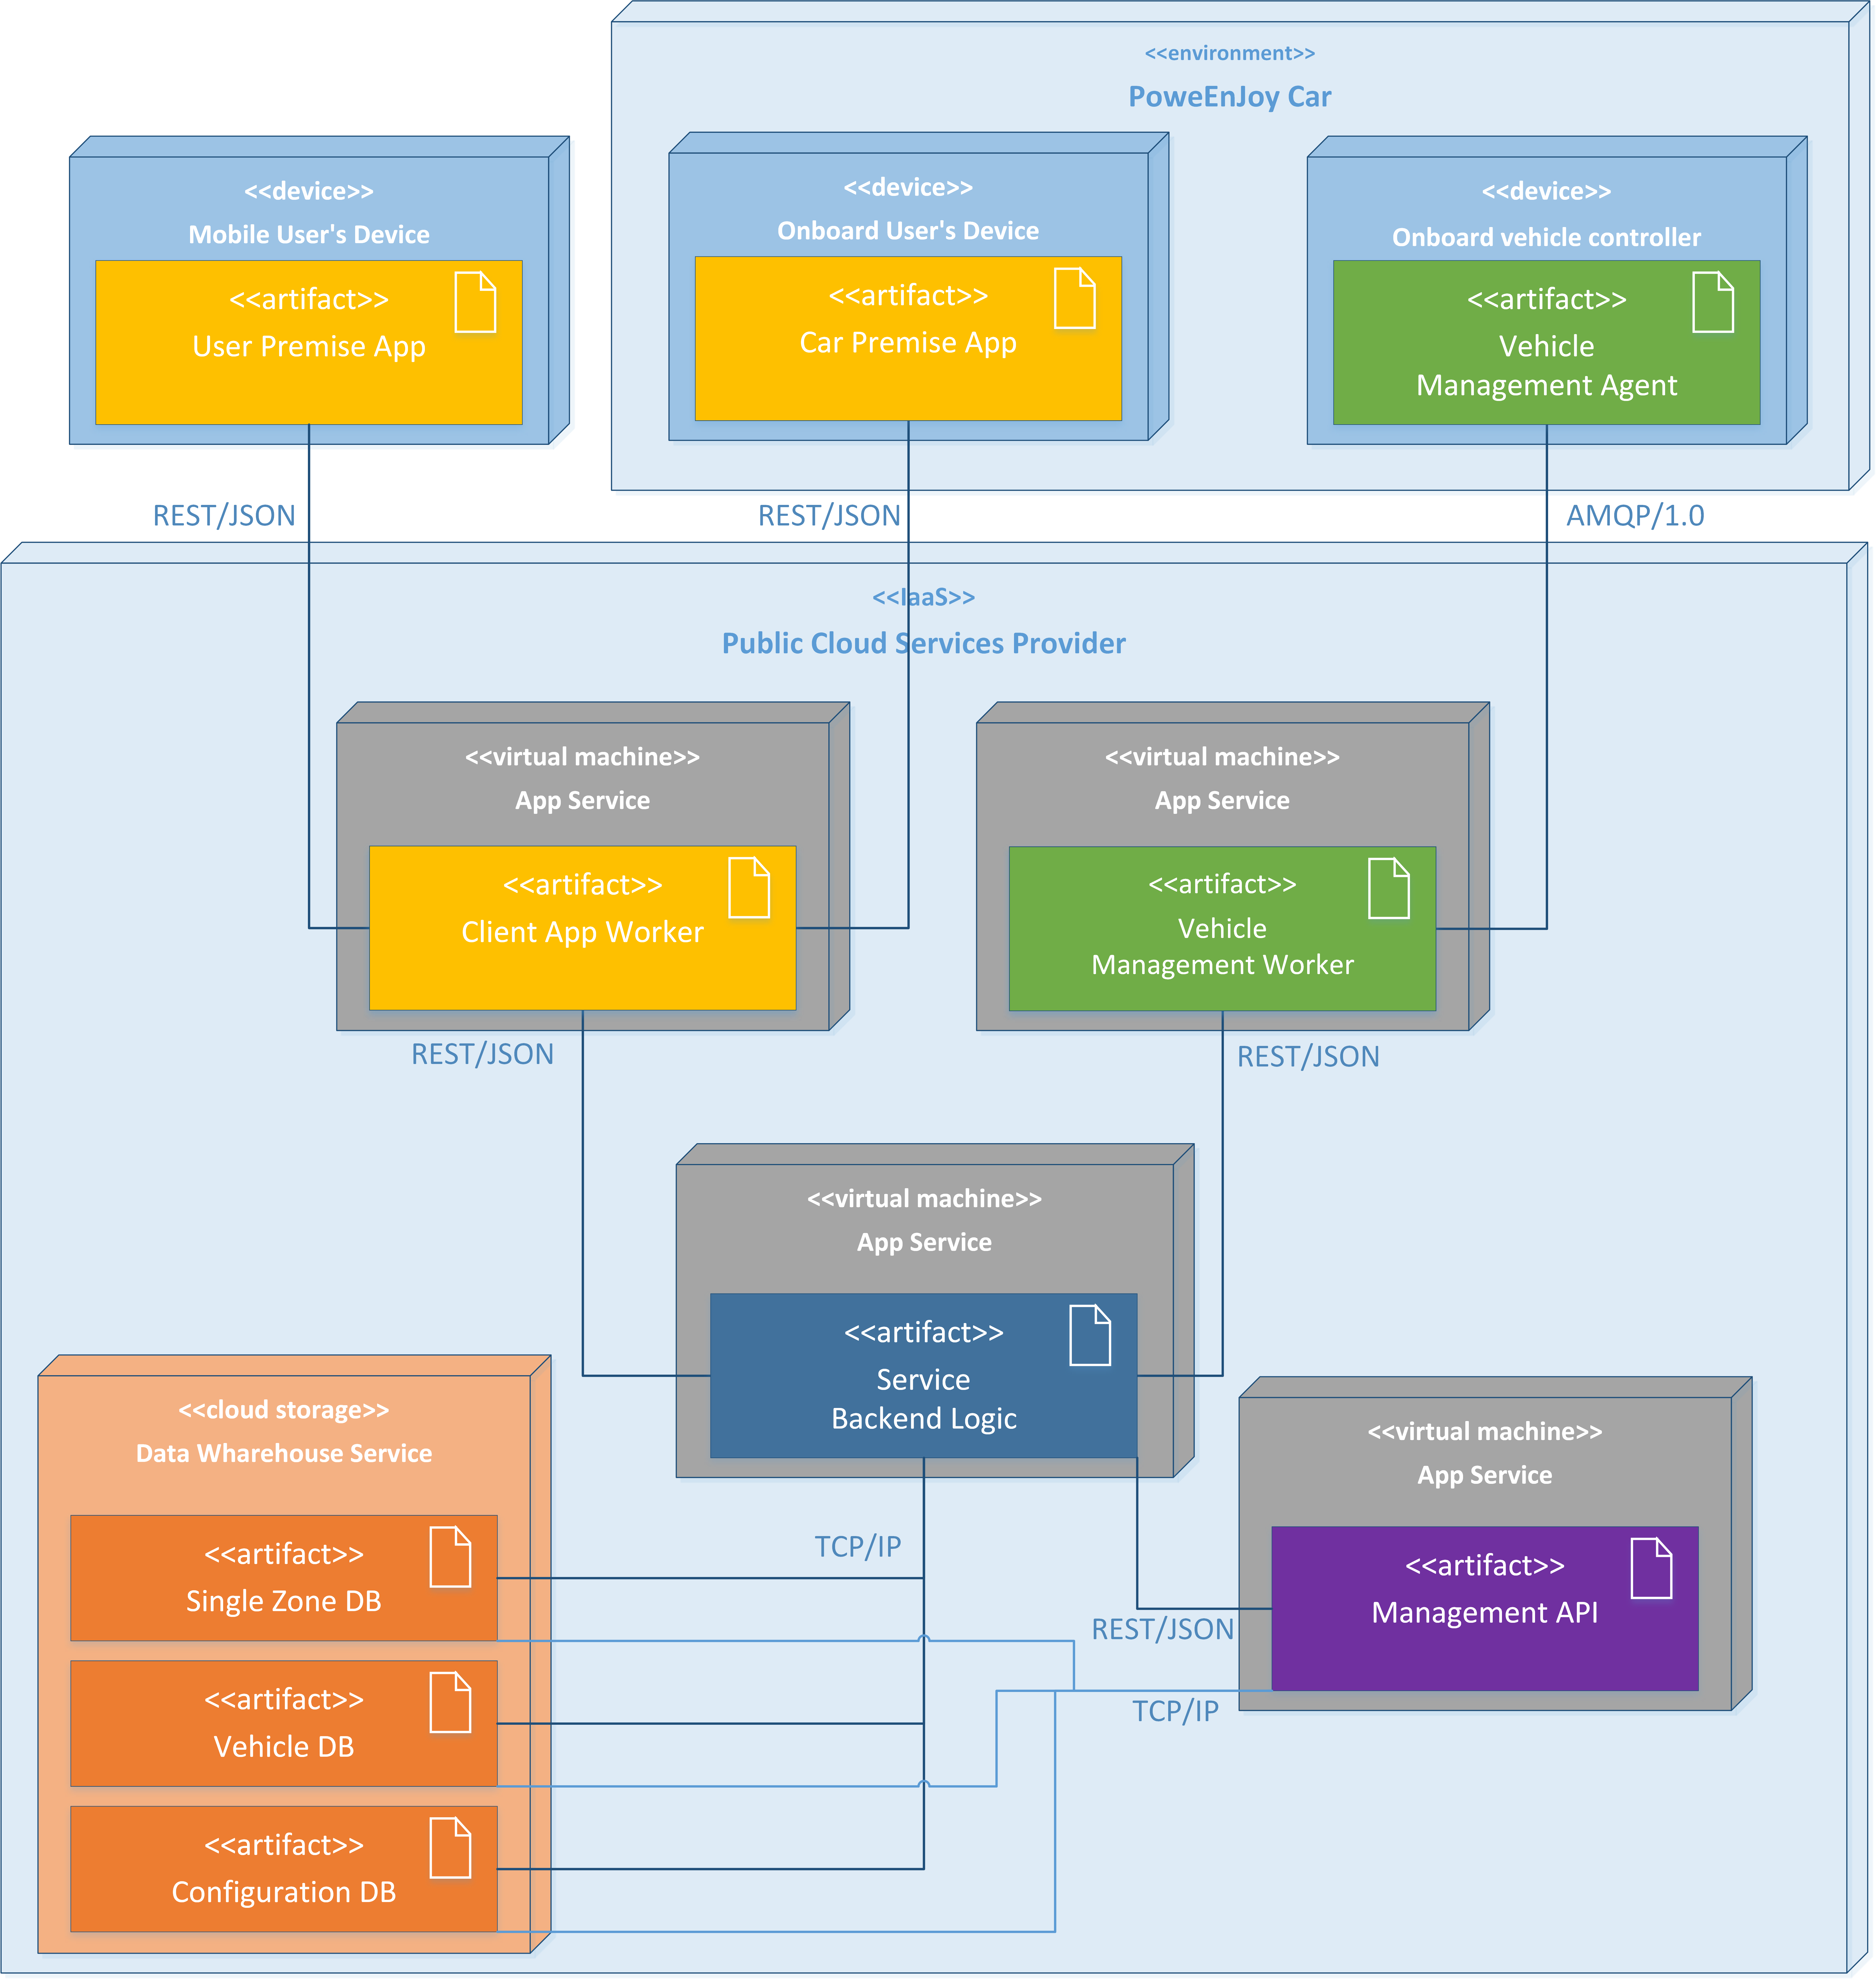
\includegraphics[scale=0.51]{{Figures/Deployment.png}}
\label{fig:Deployment}
\end{figure}
EXPLANATION TEXT
%Add \newpage here if necessary
\newpage


\subsection{Runtime view}

This section contains some Sequence Diagrams of the application.\\
In particular it shows what happens whenever:
\begin{itemize}
\item User send a request for unlock the Car;
\item User set ride destination and drive towards it; \newline
    the third diagram extends the second one and shows the Special Parking Area List and the Money Saving option features.
\end{itemize}

\newpage

\begin{landscape}
\begin{figure} [h!]
\centering
\includegraphics[scale=0.6]{{Figures/Sequence_Diagram/CarUnlock.png}}
\label{fig:UML Sequence Diagram: Car unlocking}
\caption{Car Unlocking}
\end{figure}
\end{landscape}

\newpage
\begin{landscape}
\begin{figure} [h!]
\centering
\includegraphics[scale=0.6]{{Figures/Sequence_Diagram/Ride.png}}
\label{fig:UML Sequence Diagram: Ride}
\caption{User's ride}
\end{figure}
\end{landscape}

\newpage

\begin{figure} [h!]
\centering
%scale=0.46
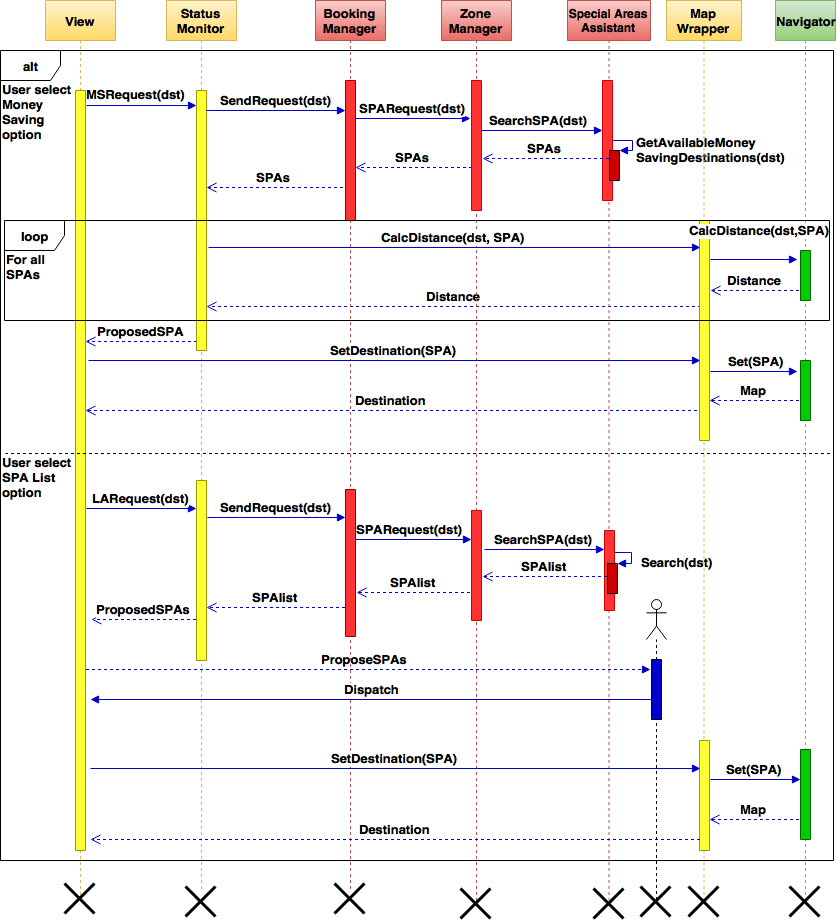
\includegraphics[scale=0.55]{{Figures/Sequence_Diagram/MS.png}}
\label{fig:UML Sequence Diagram: Money Saving and List Parking Area options}
\caption{Money Saving and List Parking Area options}
\end{figure}

\newpage

\subsection{Component interfaces}

\subsection{Selected architectural styles and patterns}

\subsection{Other design decisions}